\chapter{Problem domain analysis}\label{ch:problemanalysis}

This chapter contains a problem domain analysis of how Labelless Medias handles requests. So, the purpose of the chapter is to identify and model the problem domain.


The problem analysis will be done by applying the FACTOR and PACT analysis methods on the case, formulated by Labelless Media. Following the system definition, an analysis of both the problem domain and the application domain will be given. The output of these analyses will be used to ensure, that the system development will conform to the requirements given by Labelless Media.




%%% Application Domain Analysis %%%
\section{Application domain analysis}

\subsection{Actors}
To get a better understand of the system's users an overview and their possible usage of the system is made. The system has 2 actors and they are the members and admins. The only difference between the two actors is that only an admin can remove and create members.
\newline \newline \noindent
For both actors the user experience starts with opening the webpage and logging in. If the login gets rejected, it returns to the login page, otherwise it opens the member part of the webpage. From here the member can administrate the filter, clients and requests. After the member finishes their current tasks, they can either close the webpage and end the session, or log off and return to the login page. The member may close the webpage at any time during the session.
\newline
\begin{figure}[H]
    \centering
    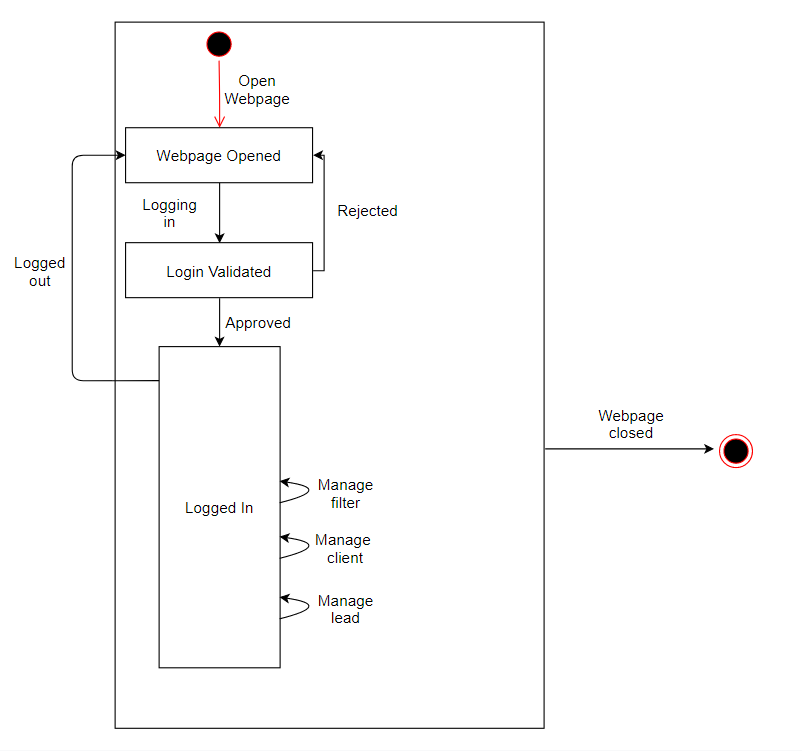
\includegraphics[scale=.7, clip]{figures/useCaseMember.png}
    \caption{Statechart diagram for a member}
    \label{fig:useCaseMember}
\end{figure}
\noindent
Like the member, the admin is able to manage the filter, clients and requests. The difference between member and admin is that the admin can also manage members. This role is created in order to add and remove new members if necessary. 
\begin{figure}[H]
    \centering
    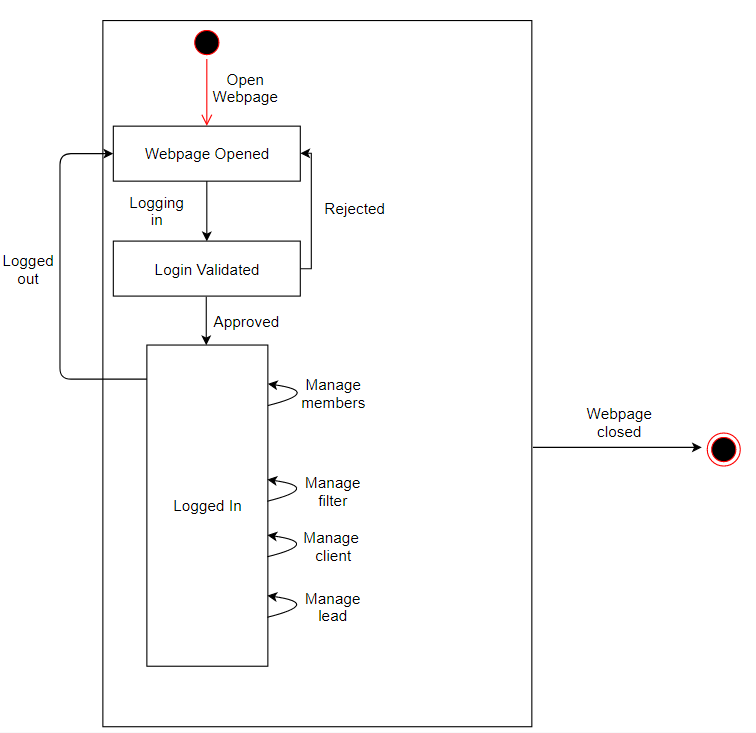
\includegraphics[scale=.7, clip]{figures/useCaseAdmin.png}
    \caption{Statechart diagram for an admin}
    \label{fig:useCaseAdmin}
\end{figure}

\subsection{Usage}
To get a better understanding of how the actors use the system, a table of use cases and actors is created.
The table illustrates the use cases and which actors are involved in the different use cases.
As seen in Figure \ref{tab:useCaseTable}, most of the use cases are relevant 
\newline \newline \noindent
\textbf{Use cases}\newline
Mangler der ikke noget her???
\begin{table}[]
\begin{tabular}{|l|l|l|}
\hline
\textbf{Use cases}                  & Admin & Member \\ \hline
Login                      & X     & X     \\ \hline
Accept request             & X     & X      \\ \hline
Deny request               & X     & X      \\ \hline
Change request icon        & X     & X      \\ \hline
Change request description & X     & X      \\ \hline
Finish request             & X     & X      \\ \hline
Change password            & X     & X      \\ \hline
Manage filter criteria     & X     & X      \\ \hline
Add member                 & X     &       \\ \hline
Remove member              & X     &       \\ \hline
Add new contact person     & X     & X      \\ \hline
\end{tabular}
\caption{Table over use cases, and their relation to the actors.}
\label{tab:useCaseTable}
\end{table}
\newpage
\noindent
\textbf{Login}\newline
Every time the web application opens, the user is prompted with a login page. The reason for this is to prevent unwanted people accessing the web application. The web application contains data that only the staff at Labelless Media is supposed to see. The use case for login can be seen in Figure \ref{fig:useCaseLogin}.
\begin{figure}[H]
    \centering
    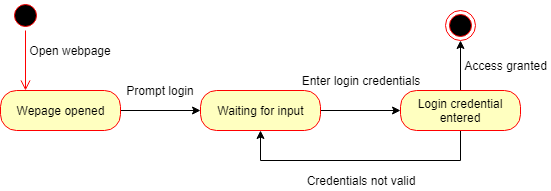
\includegraphics[scale=0.6, clip]{figures/useCaseLogin.png}
    \caption{Use case for login }
    \label{fig:useCaseLogin}
\end{figure}
\noindent
\textbf{Change request icon}\newline
During the lifetime of a request, it can change between different stages. These stages are illustrated by icons. All users are allowed   to change the stage for the requests. A request stage can be updated several times. The use case for a request can be seen in Figure \ref{fig:useCaseChangeRequestIcon}.
\begin{figure}[H]
    \centering
    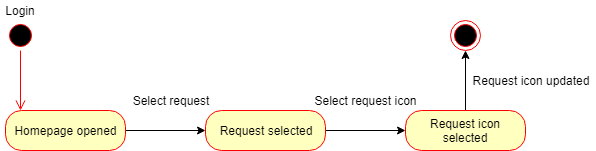
\includegraphics[scale=0.6, clip]{figures/useCaseChangeRequestIcon.png}
    \caption{Use case for changing the request icon}
    \label{fig:useCaseChangeRequestIcon}
\end{figure}
\noindent
\textbf{Finish request}\newline
When a request is done, a member has to mark it as finished in the system which is shown in Figure \ref{fig:useCaseFinishRequest}. When a request is marked as finished, the user is prompted with a review form where the user evaluates the job. When the request is reviewed, the icon of the request is updated, and the request is marked as finished in the system.
\begin{figure}[H]
    \centering
    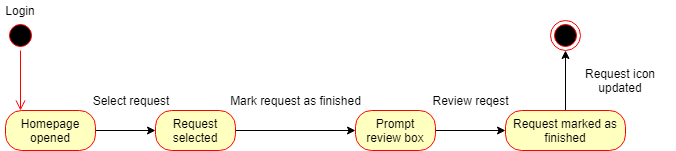
\includegraphics[scale=0.6, clip]{figures/useCaseFinishRequest.png}
    \caption{Use case for finishing a request}
    \label{fig:useCaseFinishRequest}
\end{figure}
\noindent
\textbf{Change password for member}\newline
Whenever a member is logged in, the member is able to change its password. In order to change the password, the member has to type in the current password for validation.
\begin{figure}[H]
    \centering
    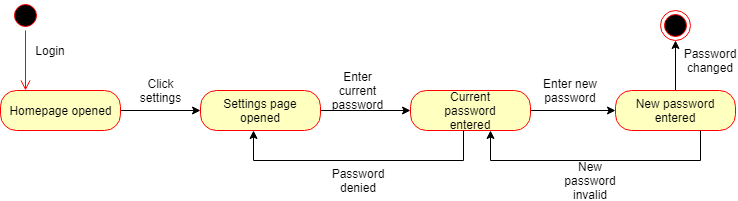
\includegraphics[scale=0.6, clip]{figures/useCaseMemberChangePassword.png}
    \caption{Use case for a member password change}
    \label{fig:useCaseMemberChangePassword}
\end{figure}
\noindent
\textbf{Change password as admin}\newline
An admin is able to change password for all users in the system. When an admin changes a password for a user, the admin must enter his own password as validation. 
\begin{figure}[H]
    \centering
    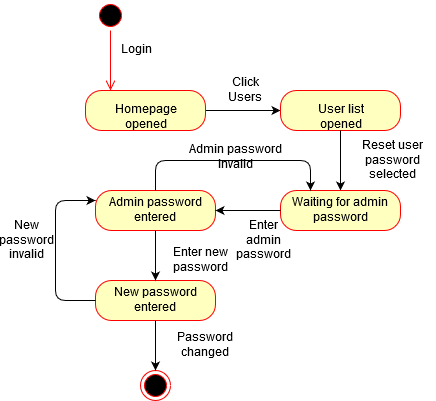
\includegraphics[scale=0.6, clip]{figures/useCaseChangePasswordAdmin.png}
    \caption{Use case for an admin password change}
    \label{fig:useCaseAdminChangePassword}
\end{figure}
\noindent
\textbf{Add member}\newline
When a new member has to be added to the system, an admin has to go through the process in Figure \ref{fig:useCaseAddMember}. First the admin goes to his homepage, and selects the member list. Then the admin inputs the relevant member data, and creates the new member.
\begin{figure}[H]
    \centering
    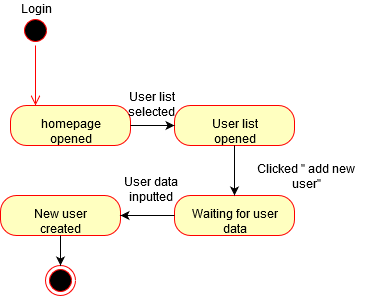
\includegraphics[scale=0.7, clip]{figures/useCaseAddMember.png}
    \caption{Use case for adding a new member}
    \label{fig:useCaseAddMember}
\end{figure}
\newpage

\subsection{Functions}
In this section the functions of the system will be identified and described. The focus of this section is what the system can do to assist the actors in their work. The functions are listed in Table \ref{tab:functionTable}, where their complexity and function type is given.
\begin{table}[H]
\begin{tabular}{|l|l|l|}
\hline
\textbf{Function name}  & \textbf{Complexity} & \textbf{Function type} \\ \hline
Login                             & Simple     & Update        \\ \hline
Log out                           & Simple     & Update        \\ \hline
Add member                        & Medium     & Update        \\ \hline
Remove member                     & Simple     & Update        \\ \hline
Change password                   & Simple     & Update        \\ \hline
Change request icon               & Simple     & Update        \\ \hline
Finish request                    & Complex    & Update        \\ \hline
Deny request                      & Simple     & Update        \\ \hline
Mark request as contacted         & Simple     & Update        \\ \hline
Show request information          & Medium     & Read          \\ \hline
Show client information           & Medium     & Read          \\ \hline
Add contact person to client      & Simple     & Update        \\ \hline
Remove contact person from client & Simple     & Update        \\ \hline
Change display criteria           & Complex    & Read          \\ \hline
Add elements to blacklist         & Simple     & Update        \\ \hline
Remove elements from blacklist    & Simple     & Update        \\ \hline
\end{tabular}
\caption{Table over functions, their complexity and types.}
\label{tab:functionTable}
\end{table}
\noindent
The complex functions from the Table will be described below, to get a better understanding of how they work. 

\textbf{Finish request}
\textbf{Change display criteria}

%%% PACT Analysis %%%
\section{PACT Analysis}
%%%%%%%%%%%%%%%%%%% INTRODUKTION  %%%%%%%%%%%%%%%%%%%%%%%%%%%%%%%%%%%%%
In this section there will be conducted a PACT analysis in order to understand the users and their requirements for the system.

\subsection{People}
The intended users of the system are the sales personnel at Labelless Media. They are experienced with managing requests, being in communication with clients, and used to using computerized systems, but with limited IT knowledge. The sales personnel all know Danish and English, but they have a strong preference towards the use of danish. The sales personnel is the primary contact with the clients, and also have other responsibilities than contacting the clients about the requests. Therefore it is important that the request system is simple, to minimize the time the sales personnel use to handle the requests. 
\newline \noindent
\textcolor{blue}{FORKLAR FORSKELLEN MELLEM DEN GAMLE PROCESS OG DEN NYE PROCESS.}


\subsection{Activities}
The overall purpose is to simplify the request managing process and thus save time for the sales personnel. Currently, the sales personnel receives an email with a request. The sales personnel then evaluates the request and determines whether or not Labelless Media should accept the request. According to the sales personnel this is a time consuming process and therefore they would like to have a system which helps them manage and process the requests. The system is supposed to give an overview over accepted, not accepted and finished request. The system is also supposed to give the requests a score, based on how attractive it seems to Labelless Media. The sales personnel is using a different system to organize the order status after they have accepted a request. This means that this system only covers the part of the process up until the clients of the requests is contacted. When Labelless Media has produced the product for the client, the system allows sales personnel to review the working process and then mark the request as finished.

\subsection{Context}
The sales personnel are working at the physical location of the company which allows them to discuss the requests with other employees of the company. 

\subsection{Technologies}
Currently the sales person uses only Mac, with external screens varying sizes. Thus the system should be scalable to fit the different screen sizes. The system will be developed as web app and will thus be accessible on all current OS and various devices with internet access and modern browsers. 


\section{Requirements}
This section contains the requirements for the system. The requirements are split into two categories; functional and non-functional requirements. The functional requirements is what system must be able to do. The non-functional requirements are the qualities the system must have. The different requirements will be categorised by using the MoSCoW rules. These rules categorises the requirements into four categories. 

\begin{itemize}
    \item Must have
    \item Should have
    \item Could have
    \item Want to have, but won't be implemented. 
\end{itemize}

\subsection{Functional requirements}
\textbf{Must have}
\begin{table}[H]
\begin{tabular}{|l|l|}
\hline
Iteration & Requirement \\ \hline
I0        & Example     \\ \hline
I0        & Example     \\ \hline
\end{tabular}
\end{table}
\noindent
\textbf{Should have}
\begin{table}[H]
\begin{tabular}{|l|l|}
\hline
Iteration & Requirement \\ \hline
I0        & Example     \\ \hline
I0        & Example     \\ \hline
\end{tabular}
\end{table}
\noindent
\textbf{Could have}
\begin{table}[H]
\begin{tabular}{|l|l|}
\hline
Iteration & Requirement \\ \hline
I0        & Example     \\ \hline
I0        & Example     \\ \hline
\end{tabular}
\end{table}
\noindent
\textbf{Want to have}
\begin{table}[H]
\begin{tabular}{|l|l|}
\hline
Iteration & Requirement \\ \hline
I0        & Example     \\ \hline
I0        & Example     \\ \hline
\end{tabular}
\end{table}
\noindent
\subsection{Non-functional requirements}
\textbf{Must have}
\begin{table}[H]
\begin{tabular}{|l|l|}
\hline
Iteration & Requirement \\ \hline
I0        & Example     \\ \hline
I0        & Example     \\ \hline
\end{tabular}
\end{table}
\noindent
\textbf{Should have}
\begin{table}[H]
\begin{tabular}{|l|l|}
\hline
Iteration & Requirement \\ \hline
I0        & Example     \\ \hline
I0        & Example     \\ \hline
\end{tabular}
\end{table}
\noindent
\textbf{Could have}
\begin{table}[H]
\begin{tabular}{|l|l|}
\hline
Iteration & Requirement \\ \hline
I0        & Example     \\ \hline
I0        & Example     \\ \hline
\end{tabular}
\end{table}
\noindent
\textbf{Want to have}
\begin{table}[H]
\begin{tabular}{|l|l|}
\hline
Iteration & Requirement \\ \hline
I0        & Example     \\ \hline
I0        & Example     \\ \hline
\end{tabular}
\end{table}

%%%%%%%%%%%%%%%%%%%%%%%%%%%%%%%%%%%%%%%%%%%%
%Figure \ref{fig:behaviourReview} illustrates a state diagram of a review object. Following the creation of a review, it will be linked to its corresponding order. When the review has been created, it is possible to edit it. The review will only cease to exist when either it or its order is deleted.
%\begin{figure}[H]
    %\centering
   % \includegraphics[scale=1, clip]{figures/reviewBehaviour.png}
  %  \caption{The behaviour of a review }
 %   \label{fig:behaviourReview}
%\end{figure}
%
%%%%%%% LEGACY RAPPORT, SKAL RYKKES TIL TRASH, NÅR Lead erns the client's answers to the questions in the contact form that is found on Labelless Media's website, see Chapter \ref{ch:case} for more information about the form. This information is used to evaluate the attractiveness of the request. The attractiveness helps Labelless Media to determine whether or not they want to accept the request. The object of Request also contains the information about whether or not the clients has been contacted about the request. If the request is accepted it changes into an order, and if it gets denied the request gets marked as denied.
%\subsection{Order}
%The Order class is a continuation of the Request class. A request becomes an order, when Labelless Media accepts the request. This change indicates, that the request has now become a project Labelless Media is working on. An order can be in various stages after it is created. Most of these stages fall outside of the system scope, and will not be described here. In this system, it is only important to keep track of when an order is accepted, and when it is completed. When the order has been completed, a review of the order has to be filed. An order can also be cancelled after it has been created. When an order is cancelled, it will still be possible to review it, and the order will stay in the archive. 

%\subsection{Review}
%% Er indsat fra client class - skal omformuleres i denne subsection.
%The reviews are created by Labelless Media, and is used to keep track of %Labelless Media's experience with the work they have done for the client.
%Figure \ref{fig:behaviourRequest} illustrates a state diagram of an object of a request which has two different states. The first state "Awaiting contact" concern a client which is still not contacted about a request. This state is also where the request gets ranked by the system. The second state is "Arranging". Here the sender of the request has been contacted, but yet to be confirmed. After this the life cycle of the request ends and it can not be changed further. If Labelless Media decides to not take the request, the life cycle will end earlier in the process.
%\begin{figure}[H]
%    \centering
%    \includegraphics[scale=0.7, clip]{figures/requestBehaviour.png}
%    \caption{The behaviour of a request }
%    \label{fig:behaviourRequest}
%\end{figure}
%
%\noindent


\noindent
%Figure \ref{fig:behaviourArchive} illustrates the behavior of the archive class. The archive can sort itself, add clients, remove clients and add leads to a client in the archive.
%Add client to archive is simply just adding a new client to the archive and remove client will remove a specified client from the archive.
%Add leads to client is used when a already existing client makes a new lead. When this happens the lead will simply be added to the already existing client
%When sorting, the archive will ask the evaluator to update the score for all the leads, to make sure that it doesn't use outdated values when sorting.

%\begin{figure}[H]
 %   \centering
  %  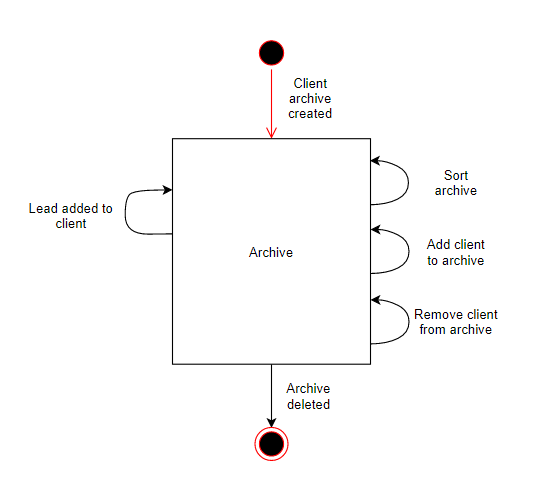
\includegraphics[scale=1, clip]{figures/archiveBehaviour.png}
  %  \caption{The behaviour of an archive }
  %  \label{fig:behaviourArchive}
%\end

%\textbf{Joblist}
%\\
%Figure \ref{fig:behaviourJoblist} illustrates the behavior of a joblist. The \textit{joblist} class represents the leads a salesperson has taken upon him. A salesperson has his own joblist, which contains all active leads. After a salesperson is hired the joblist is active. The salesperson can reserve a lead to the joblist, which permanently associates the salesperson, with the lead. The joblist can also update a lead status, which entails accepting, declining and completing a lead.

%\begin{figure}[H]
%    \centering
%    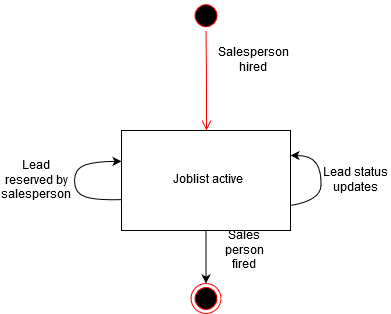
\includegraphics[scale=0.9, clip]{figures/Behaviors/BehaviorJoblist.png}
%    \caption{The behaviour of a joblist }
%    \label{fig:behaviourJoblist}
%\end{figure}